\begin{figure}[H]
\centering
\includegraphics[page=6,width=0.48\textwidth]{\FCNCFigures/xTFW/showFake/NOMINAL/reg2mtau1b2jos_vetobtagwp70_highmet/tau_pt_0.pdf}
\includegraphics[page=6,width=0.48\textwidth]{\FCNCFigures/xTFW/showFake/NOMINAL/reg2mtau1b3jos_vetobtagwp70_highmet/tau_pt_0.pdf}\\
\includegraphics[page=6,width=0.48\textwidth]{\FCNCFigures/xTFW/showFake_samesign/reg2mtau1b2jos_vetobtagwp70_highmet/tau_pt_0.pdf}
\includegraphics[page=6,width=0.48\textwidth]{\FCNCFigures/xTFW/showFake_samesign/reg2mtau1b3jos_vetobtagwp70_highmet/tau_pt_0.pdf}\\
\includegraphics[page=6,width=0.48\textwidth]{\FCNCFigures/xTFW/showFake_sideband/reg2mtau1b2jos_vetobtagwp70_highmet/tau_pt_0.pdf}
\includegraphics[page=6,width=0.48\textwidth]{\FCNCFigures/xTFW/showFake_sideband/reg2mtau1b3jos_vetobtagwp70_highmet/tau_pt_0.pdf}
\caption{STH $\thadhad$ (左)和TTH $\thadhad$(右)信号区分别使用三组FF进行Fake tau估计后的Leading $\tauhad$的$\pt$谱。其中最上方的图中使用的FF由W+jet CR控制区导出,中间的图中使用的FF由SS CR控制区导出,最下方的图中使用的FF由OS CR控制区导出。}
\label{fig:fakeEstimation_had}
\end{figure}

